\documentclass[]{article}
\usepackage[latin1]{inputenc}
\usepackage{amsmath,amssymb,bm} % math stuff
\usepackage[top=1.85cm, bottom=1.65cm, left=2.2cm, right=2.2cm]{geometry}
\usepackage{url}
% FOR DISPLAYING CODE
\usepackage{listings}
\usepackage{color}
\definecolor{dkgreen}{rgb}{0,0.6,0}
\definecolor{gray}{rgb}{0.5,0.5,0.5}
\definecolor{mauve}{rgb}{0.58,0,0.82}

\lstset{frame=tb,
	language=Python,
	aboveskip=3mm,
	belowskip=3mm,
	showstringspaces=false,
	columns=flexible,
	basicstyle={\small\ttfamily},
	numbers=none,
	numberstyle=\tiny\color{gray},
	keywordstyle=\color{blue},
	commentstyle=\color{dkgreen},
	stringstyle=\color{mauve},
	breaklines=true,
	breakatwhitespace=true,
	tabsize=4
}

% FOR FIGURES
\usepackage{tikz}
\usetikzlibrary{arrows,calc,positioning,shadows,shapes}



%opening
\title{An introductory guide to \pycle \\
	\large (the \textbf{Py}thon \textbf{c}ompresive \textbf{le}arning toolbox)}
\author{Vincent Schellekens}

\newcommand{\code}{\texttt}
\newcommand{\pycle}{\code{pycle}}
\renewcommand{\Vec}[1]{\bm{#1}} % Pour les vecteurs, re if using amsmath
\newcommand{\bb}{\mathbb}

\begin{document}

% TODO 
% - link to matlab toolbox

\maketitle

\begin{abstract}
	This guide presents \pycle: a Python toolbox to perform compressive/sketched learning. It first shortly explains what ``compressive learning'' means, and how this toolbox is organized. A detailed tutorial then teaches how to use its main features. To dive in right away, some complementary practical examples are available as jupyter notebooks on the main github page of \pycle: \url{https://github.com/schellekensv/pycle}.
\end{abstract}

\section{Introduction}
\subsection{What is compressive learning?}
In usual machine learning, we fit some parameters $\theta$ (e.g., a parametric curve in regression, centroids in k-means clustering, weights in a neural network...) to a given set of training data $X$. The actual algorithms for such tasks usually necessitate to access this training set multiple times (one complete pass on the dataset is sometimes called an ``epoch''). This can be cumbersome when the dataset is extremely large, and/or distributed across different machines. Compressive learning (CL, also called sketched learning) seeks to circumvent this issue by compressing the whole dataset into one lightweight ``sketch'' vector, that requires only one pass on the dataset and can be computed in parallel. Learning is then done using only this sketch instead of the inconveniently large dataset (that can be discarded). This allows to significantly reduce the computational resources that are needed to handle massive collections of data.


		
\begin{figure}[!htb]
	\centering
	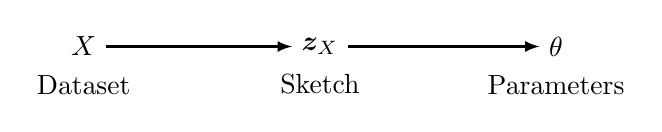
\begin{tikzpicture}
	% Place nodes
	\node [label=below:Dataset] (dataset) at (0,0) {$X$};
	\node [label=below:Sketch] (sketch) at (3,0) {$\Vec{z}_X$};
	\node [label=below:Parameters] (parameters) at (6,0) {$\theta$};
	
	% Draw edges
	\draw [->, thick, -latex] (dataset) -- (sketch);
	\draw [->, thick, -latex] (sketch) -- (parameters);
	\end{tikzpicture}
	\caption{The compressive learning workflow.}
	\label{fig:CL}
	\end {figure}

More precisely, CL comprises two steps (Figure \ref{fig:CL}):
\begin{enumerate}
	\item \textbf{Sketching:} The dataset $X = \{\Vec{x}_i \: | \: i = 1, ..., n\}$ (where we assume $\Vec{x}_i \in \bb R^d$) is compressed as a sketch vector that we note $\Vec{z}_X$, defined as the average over the dataset of some features $\Phi(\Vec{x}_i)$ (the function $\Phi : \mathbb R^d \mapsto \mathbb C^m$ or $\bb R^m$ computes $m$ features, possibly complex):
		\begin{equation}
		\label{eq:sketching}
		\Vec{z}_X := \frac{1}{n} \sum_{i = 1}^n \Phi(\Vec{x}_i).
		\end{equation}
	Since this is a simple averaging, sketching can be done on different chunks of $X$ independently, which is quite handy in distributed or streaming applications.
	\item \textbf{Learning:} The target model parameters $\theta$ are then obtained by some algorithm $\Delta$ that operates \emph{only} on this sketch,
		\begin{equation}
			\theta = \Delta(\Vec{z}_X).
		\end{equation}
		Typically, this involves solving some optimization problem $\min_{\theta} f(\theta ; \Vec{z}_X)$.
\end{enumerate}

\noindent In the following, these steps are explained intuitively, the formal details being introduced only when needed; for a more solid/exhaustive overview of compressive learning, see \cite{gribonval2017compressive}.

% TODO explain how it is structured, how to use


\subsection{Requirements}
The \pycle~package is built on standard Python scientific computing libraries: \code{numpy}, \code{scipy} and \code{matplotlib}; if you don't already have them installed, follow the instructions at \url{https://www.scipy.org/install.html}. %

% todo latest versions?

% You can install those packages by...

\subsection{Toolbox organization}
The \pycle~toolbox is a collection of several submodules:
\begin{enumerate}
	\item The \code{sketching.py} module instantiates feature maps then computes the sketch of datasets with it.
	\item The \code{compressive\_learning.py} module contains the actual ``learning'' methods, extracting the desired parameters from the sketch.
	\item The \code{utils.py} module contains miscellaneous auxiliary functions, amongst others for generating synthetic datasets and evaluate the obtained solutions (as well quantitatively with well-defined metrics as qualitatively with visualization tools).
	\item Finally, the \code{third\_party.py} module serves to group code chunks used by \pycle that are written by other developers but not published as independent packages.
\end{enumerate}



\section{A tutorial tour of \pycle}
Let's explore the core submodules of \code{pycle}! Our focus here is understanding, so this section is a high-level tutorial rather than an exhaustive enumeration of what's inside the toolbox. %(however, section \ref{sec:documentation} is a methodical list of all the toolbox features). 

\subsection{Sketching datasets with the \code{sketching.py} submodule} 
To use the \code{sketching} submodule, you first need to import it; I often use \code{sk} as shorthand. Sketching, as defined in~\eqref{eq:sketching}, is done by simply calling \code{sk.computeSketch}, as follows (we'll fill in the dots later):
\begin{lstlisting}
import pycle.sketching as sk # import the sketching submodule

X = ...    # load a numpy array of dimension (n,d)
Phi = ... # sketch feature map, see later

z = sk.computeSketch(X,Phi) # z is a numpy array containing the sketch
\end{lstlisting}

\noindent As shown in the code snippet, \code{sk.computeSketch} requires two arguments: the dataset $X$ (given as a numpy array of dimensions $(n,d)$) and the feature map $\Phi$, which must be an instance of a \code{sk.FeatureMap} object\footnote{
Why do we use \code{FeatureMap} objects instead of (Python) functions to represent... well, (mathematical) functions? The reason is that we often require additional information about $\Phi$ (such as the ambient dimension $d$, the target dimension $m$, a method to compute the jacobian $\nabla\Phi$,...). All these parameters and methods are thus conveniently packaged inside the \code{FeatureMap} objects.}. %Let's start with the simplest one: the dataset $X$ should be given as a 2-d numpy array of dimensions $(n,d)$, i.e., number of examples times their dimension\footnote{\textbf{Matrix representation conventions:}
%We follow the same convention as most mainstream Python machine learning modules: the dataset, mathematically described as $X = (\Vec{x}_i \in \mathbb R^d)_{i = 1}^n \in \mathbb R^{d \times n}$, is represented by a numpy array of shape $(n,d)$. In particular, \code{X[0]} references $\Vec{x_1}$: note the awkward inversion of dimension order. For matrices that don't represent datasets (e.g., $\Omega$ in the examples below), we stick to the mathematical convention instead, i.e., a matrix of the type $\mathbb R^{a \times b}$ is represented by a numpy array of shape $(a,b)$.}.
%The feature map argument can be specified in one of the two following ways. Either---and this is the method I recommend---you give an instance of a \code{FeatureMap} object (explained below), or you directly provide a callable Python function (e.g., to compute the second-order moments for the sketch, write \code{Phi = lambda x: x**2}). Note that the second method is proposed for research purposes, in the case you want to construct a custom feature map that cannot be instantiated with the methods provided within the \code{FeatureMap} class\footnote{\textbf{FeatureMap objects:}
%Why do we use \code{FeatureMap} objects instead of (Python) functions to represent... well, (mathematical) functions? Because we often require additional metadata/methods about $\Phi$ (e.g., target dimension $m$, jacobian $\nabla\Phi$,...). All these parameters and methods are conveniently packaged inside \code{FeatureMap} objects.}.
%\emph{Voil�}, you know the basics of how the \code{sketching} submodule is used! Well, OK, all we saw was a function that computes an average, but hey, that's like, the essence of sketching, it's not my fault. Luckily for you, \code{sketching} has much more to offer. First and foremost, I'll demonstrate the whole zoo of feature maps that are readily available---I promise you, you'll construct your \code{FeatureMap} object $\Phi$ in no more than two lines of code. After this comes more advanced methods of the toolbox that you may not need right away: I'll show how to automatically select the \emph{scale hyper-parameter} in the aforementioned feature maps (which in practice can be hard to guess \emph{a priori}); I'll then finally explain \code{pycle}s functions for sketching with Differential Privacy guarantees. 
%\subsubsection{Painless instantiation of standard feature maps: the \code{SimpleFeatureMap} class}
Actually, all feature maps used up to now in CL are of the following ``Simple Feature Map'' form:
\begin{equation}
\Phi(\Vec{x}) = f(\Omega^T\Vec{x} + \Vec{\xi}), \quad \text{where} \quad \Omega = [\Vec{\omega}_1, \cdots, \Vec{\omega}_m] \in \mathbb{R}^{d \times m}, \: \Vec{\xi} = [\xi_1, \cdots, \xi_m]^T \in \mathbb{R}^{m},
\end{equation}
and $f$ is a point-wise nonlinearity (i.e., $\Phi_j(\Vec{x}) = f(\Vec{\omega}_j^T\Vec{x} + \xi_j)$ for all $j$)\footnote{One way to interpret this map is to associate it with a one-layer neural network (without learning the ``weights'' $\Omega$).}.  You can easily instantiate such a nonlinearity in \code{pycle} using the a \code{SimpleFeatureMap} child class:
\begin{lstlisting}
import pycle.sketching as sk

f = ...       # nonlinearity (Python function, tuple or string)
Omega = ...   # (d,m) numpy array
xi = ...      # (m,) numpy array
Phi = sk.SimpleFeatureMap(f, Omega, xi)
\end{lstlisting}

We now explain how to set those three arguments.
\begin{itemize}
	\item \textbf{Nonlinearity \code{f}:} you can simply pass as a string the name of standard nonlinearities used in CL, such as:
	\begin{itemize}
		\item \code{"complexExponential"}, for the complex exponential $f(\cdot) = \exp(\mathrm i \cdot)$ (corresponds to the random Fourier features sketch);
		\item \code{"cosine"}, simply the cosine $f(\cdot) = \cos(\cdot)$ (the real part of the random Fourier features sketch);
		\item \code{"universalQuantization"}, for the one-bit square wave with normalization in $\{\pm 1\}$, given by $f(\cdot) = \mathrm{sign} \circ \cos(\mathrm \cdot)$ and used for quantized sketching~\cite{schellekens2018quantized}. The ``complex equivalent'' is also available, under the name of \code{"universalQuantization\_complex"}, which corresponds to $f(\cdot) = \mathrm{sign} \circ \cos(\mathrm \cdot) + \mathrm{i} \cdot \mathrm{sign} \circ \sin(\mathrm \cdot)$.
	\end{itemize}
	Alternatively, you can pass in any Python function $\bb R \mapsto \bb C$ or $\bb R$. However, since computing the gradient\footnote{Noting the Jacobian matrix $\nabla \Phi(\Vec{x}) = [\nabla \Phi_1(\Vec{x}) , \cdots , \nabla \Phi_m(\Vec{x}) ] \in \bb R^{d \times m}$ and $f'(t) = \frac{\mathrm{d}f(t)}{\mathrm{d}t}$ applied component-wise, we have $ \nabla \Phi(\Vec{x}) = \mathrm{diag} \left( f'(\Omega^T \Vec{x} + \Vec{\xi})\right) \cdot \Omega.$} $\nabla\Phi$ requires $\frac{\mathrm{d}f(t)}{\mathrm{d}t}$, you can also pass in a \emph{tuple} of functions $(f,\frac{\mathrm{d}f(t)}{\mathrm{d}t})$ in order to use gradient-based CL methods later. 
	\item \textbf{Projections/frequencies \code{Omega}:} A $(d,m)$ numpy array, typically randomly generated. Without entering into the details, common choices are instantiated by \code{sk.drawFrequencies(drawType,d,m,Sigma)}, where \code{drawType} is a string describing the sampling pattern (\code{Gaussian}, and \code{FoldedGaussian} or \code{AdaptedRadius} which perform better in higher dimensions, see~\cite{keriven2018sketching}) and \code{Sigma} is the associated scale parameter (in the simplest case, it is a scalar parameter corresponding to the bandwidth $\sigma^2$ of the associated Gaussian kernel).
	\item \textbf{Dither \code{xi}:} this optional parameter expects an $(m,)$ numpy array (not providing anything is equivalent to setting $\Vec\xi = \Vec 0$). To draw \emph{i.i.d.} values uniformly from $[0,2\pi]$, you can use \code{sk.drawDithering(m)}.
\end{itemize}

To summarize, here is a typical example of the creation of a sketch:

\begin{lstlisting}
import pycle.sketching as sk

# Load the dataset
X = ...    
(n,d) = X.shape

# Instantiate the feature map
m = 10*d # Sketch size
Omega = sk.drawFrequencies("FoldedGaussian",d,m,Sigma = 0.01) # Kernel bandwidth = 0.1
Phi = sk.SimpleFeatureMap("complexExponential", Omega) # No dithering used here

# Compute the sketch
z = sk.computeSketch(X,Phi) # z is a numpy array containing the sketch
\end{lstlisting}

\subsection{Learning from the sketch with the \code{compressive\_learning.py} submodule} 
For now, \pycle~features mainly one algorithm called \code{CLOMPR}. It has been proposed to estimate mixtures of Gaussians~\cite{keriven2018sketching} and to perform k-means clustering~\cite{keriven2017compressive2}. In \pycle, it is called as follows:

\begin{lstlisting}
import pycle.compressive_learning as cl

# Beforehand, define the feature map Phi and compute the sketch z

# Bounds for the data
bounds = np.array([X.min(axis=0),X.max(axis=0)])

# Define the task
task_name = ... # See below, either "k-means", "GMM" or "GMM-nondiag"
K = ... # Number of centroids/gaussian modes

# Learn from the sketch
theta = cl.CLOMPR(task_name,z,Phi,K,bounds)

# Do something with the model (prediction, visualization, ...)
\end{lstlisting}

The first argument \code{task\_name} defines the task to solve, which conditions the format of the output \code{theta}. Currently, the available options are 
\begin{itemize}
	\item \code{task\_name = "k-means"}, used to estimate the centroids of k-means clusters. In this case, \code{theta = (alpha,C)} is a tuple, where \code{alpha} contains the weights of the clusters and \code{C} its centroids (in a $(K,d)$ numpy array).
	\item \code{task\_name = "GMM"} or \code{"GMM-nondiag"}, used to fit a mixture of Gaussians to the data. Here, \code{theta = (w,mus,covs)} is a tuple of three elements, where \code{w} are the mixture coefficients, and \code{mus} and \code{covs} are the centers (resp. covariance matrices) of the Gaussian modes, in a $(K,d)$ numpy array (resp. $(K,d,d)$ numpy array). The difference between the two options is that \code{"GMM"} assumes diagonal covariance matrices, while \code{"GMM-nondiag"} improves the fit by considering general covariance matrices, during a post-processing fine-tuning step.
\end{itemize}

Detailed examples of those tasks are available on the main github page of the \pycle~toolbox. With that and the documentation\footnote{Just type \code{help(nameOfAFunction) if you want to see all the available options.}} of the different functions, you should have a good idea of how to use the toolbox in practice. In the next section, some advanced functionalities of the toolbox are described. 


\section{Advanced features of \pycle}

\subsection{Helpful tools from the \code{utils.py} submodule}

\subsubsection*{Dataset generation tools}
Several methods allow to generate synthetic datasets, the most notable being \code{generatedataset\_GMM} for datasets sampled from Gaussian mixture models (with a large set of tunable parameters). Moreover, other toy examples datasets can be generated with \code{generateCirclesDataset}, \code{generateSpiralDataset} and \code{generatedataset\_Ksparse}.

\subsubsection*{Performance metrics}
The toolbox provides several metrics to assess the quality of the learned models. For k-means, \code{SSE} computes the Sum of Squared Errors of a set of centroids. For Gaussian Mixture Models, \code{loglikelihood\_GMM} assesses the log-likelihood of the provided Gaussian mixture on a dataset. Moreover, if a ground-truth GMM is known, \code{symmKLdivergence\_GMM} estimates the (symmetrized) Kullback-Leibler divergence between two GMMs~\cite{gribonval2017compressive}.

\subsubsection*{Visualization tools}
To visualize the quality of fit of a GMM to the dataset, \code{plotGMM} plots the contour curves of the given GMMs density, along with the optional dataset.


%After this comes more advanced methods of the toolbox that you may not need right away: I'll show how to automatically select the \emph{scale hyper-parameter} in the aforementioned feature maps (which in practice can be hard to guess \emph{a priori}); I'll then finally explain \code{pycle}s functions for sketching with Differential Privacy guarantees. 
\subsection{Designing the sampling pattern parameters when drawing the feature map}
In \code{sketching.py}, a strategy to estimate \code{Sigma} (used for example in \code{sk.drawFrequencies}) from a small preliminary sketch, described in~\cite{gribonval2017compressive}, is implemented under the name \code{sk.estimateSigma}.

\subsection{Sketching with Differential Privacy}
As described in~\cite{schellekens2019differentially}, a layer of differential privacy can easily be incorporated on top of the sketch. In \pycle, this is achieved by replacing \code{computeSketch} with its variant \code{computeSketch\_DP}.



\section{Going further with \pycle}
The primary goals for the \code{pycle} toolbox are that it should be:
\begin{itemize}
	\item \textbf{intuitive to use:} practitioners with minimal knowledge in compressive learning and little experience in Python should be able to use it to implement compressive learning in their own projects;
	\item \textbf{flexible to new features:} researchers with interest in compressive learning (that want to try out new methods/techniques in CL) should be able to easily extend this code to suit their own needs, without having to re-write things from scratch (and eventually, suggesting to add some features to the toolbox);
	\item \textbf{efficient to run:} the main motivation of compressive learning is based on the fact that it can be much more memory- and time-efficient than traditional learning methods, so the performances of the toolbox should fulfill that promise (personal note: this goal is still a challenging for me, this item is rather wishful thinking). 
\end{itemize}
With this in mind, any bug reports, improvement suggestions, ideas and general comments are more than welcome: don't hesitate to contact me (\code{vincent.schellekens@uclouvain.be})! If you use the toolbox in your research, please kindly cite it using the DOI \code{10.5281/zenodo.3855114}; get BibTeX export files (or others) here: \url{https://doi.org/10.5281/zenodo.3855114}.


\newpage
\bibliography{guidebib.bib}
\bibliographystyle{ieeetr}


\end{document}
